\documentclass[10pt,journal,compsoc]{IEEEtran}
\usepackage[spanish]{babel}
\usepackage{listings}
\usepackage{graphicx}
\usepackage{wrapfig}
\usepackage{lipsum}
\usepackage[T1]{fontenc}
\usepackage{filecontents}
\ifCLASSOPTIONcompsoc
  \usepackage[nocompress]{cite}
\else
  \usepackage{cite}
\fi

\ifCLASSINFOpdf
\else
\fi
\newcommand\MYhyperrefoptions{bookmarks=true,bookmarksnumbered=true,
pdfpagemode={UseOutlines},plainpages=false,pdfpagelabels=true,
colorlinks=true,linkcolor={black},citecolor={black},urlcolor={black},
pdftitle={Curry},
pdfsubject={Lenguaje de Progemaci\'on Pascal},
pdfauthor={Daniel, Wilbert, Anthony, Bryan},
}
\renewcommand{\lstlistingname}{Cuadro}
\lstset{
	extendedchars=true,
	frame = single, 
	language=Pascal, 
	framexleftmargin=3pt
}
\hyphenation{op-tical net-works semi-conduc-tor}


\begin{document}
\title{Lisp}

\author{Daniel~Delgado,~\IEEEmembership{Estudiante,~ITCR,}
	Wilbert~Gonzales,~\IEEEmembership{Estudiante,~ITCR,}
	Anthony~Leandro,~\IEEEmembership{Estudiante,~ITCR,}
	and~Bryan~Mena,~\IEEEmembership{Estudiante,~ITCR}
}
\markboth{Lenguajes de Programaci\'on, Tarea Corta 6, Octubre 2017}
{Shell \MakeLowercase{\textit{et al.}}: \LaTex}


\maketitle

\IEEEdisplaynontitleabstractindextext

\IEEEpeerreviewmaketitle

\section{Datos Historicos}
\begin{wrapfigure}{R}{0.3\textwidth}
	\centering
	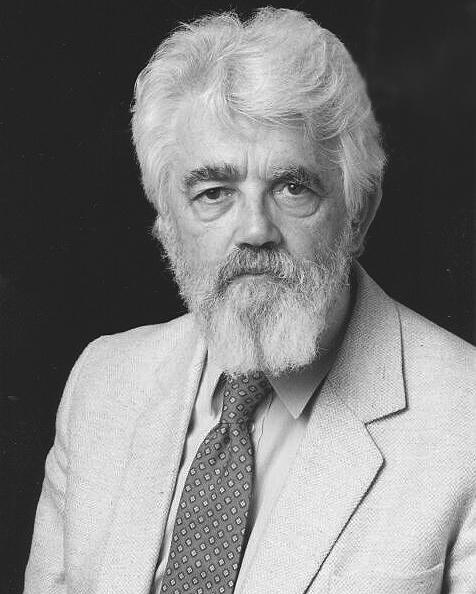
\includegraphics[width=0.25\textwidth]{mccarthy.jpg}
	\caption{\label{fig:JohnMcCarthy}John McCarthy (1927-2011).}
\end{wrapfigure}
En 1960, John McCarthy public\'o un notable art\'iculo: \emph{Funciones recursivas de expresiones simb\'olicas y su c\'omputo a m\'aquina, Parte I} (la Parte II nunca fue publicada), en el que  hizo para programar algo parecido a lo que Euclides hizo para la geometr\'ia. \'El demostr\'o c\'omo, dado un grupo de operadores simples y una notaci\'on para las funciones, se puede construir un lenguaje de programaci\'on entero. Llam\'o a este lenguaje Lisp, para "List Processing", porque una de sus ideas clave era usar una estructura de datos simple llamada \emph{lista} para c\'odigo y datos. 

\begin{wrapfigure}{R}{0.3\textwidth}
	\centering
	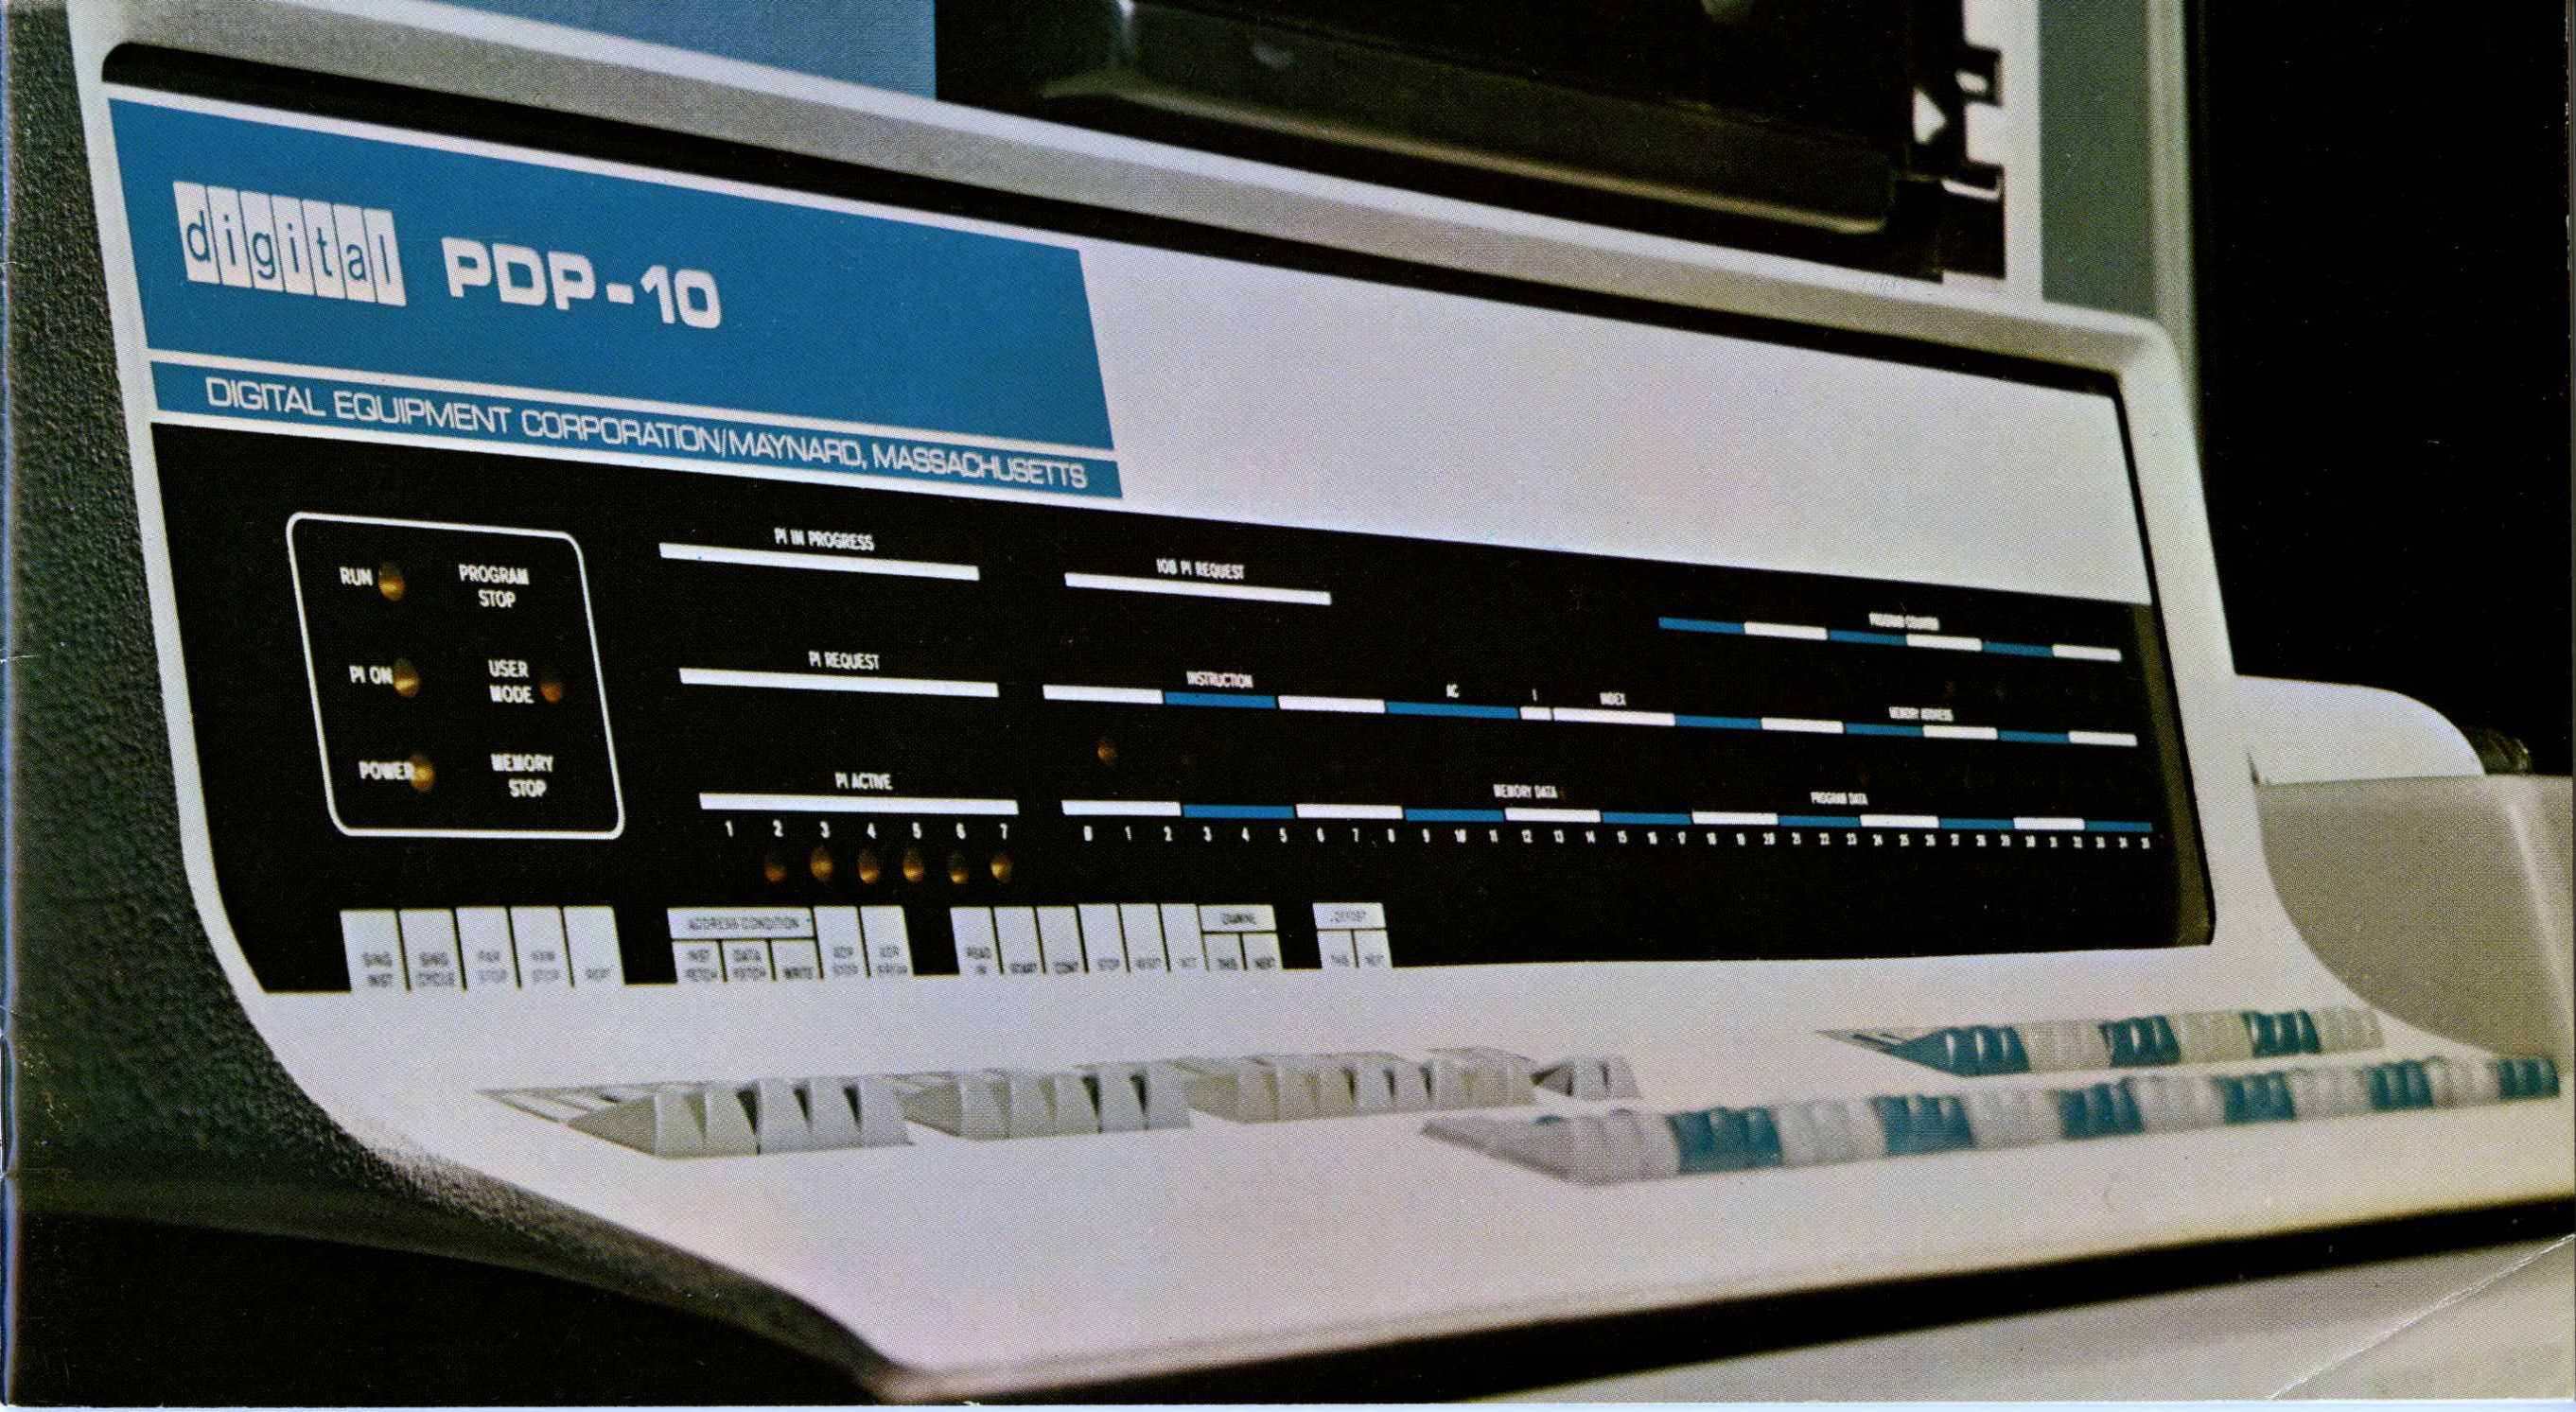
\includegraphics[width=0.25\textwidth]{pdp.jpg}
	\caption{\label{fig:PDP-10}Computador PDP-10.}
\end{wrapfigure}

Desde su inicio, Lisp estaba estrechamente relacionado con la comunidad de investigaci\'on de la inteligencia artificial, especialmente en sistemas PDP-10 (ver Figura 2). Lisp es un lenguaje multiparadigma  que utiliza \emph{notaci\'on polaca}. 

\begin{wrapfigure}{R}{0.22\textwidth}
	\centering
	
\includegraphics[width=0.12\textwidth]{s-expression.png}
	\caption{\label{fig:S-Expression}\'Arbol de Expresi\'on-S}
\end{wrapfigure}

La notaci\'on original de McCarthy usaba \emph{Expresiones-M} en corchetes que ser\'ian traducidas a \emph{Expresiones-S}. Como un ejemplo, la Expresi\'on-M \emph{car[cons[A,B]]} es equivalente a la Expresi\'on-S \emph{(car (cons A B))}. Una vez que Lisp fue implementado, los programadores r\'apidamente eligieron usar Expresiones-S, y las Expresiones-M fueron abandonadas. Una Expresi\'on-S es una notaci\'on en forma de texto, para representar una estructura de datos de \'arbol, basada en listas anidadas, en donde cada sublista es un sub\'arbol (ver Figura 3).

\section{Tipos de Datos}


\subsection{Integer}
N\'umeros sin parte fraccionaria. El rango de valores de un entero depende de la m\'aquina. El intervalo m\'inimo es de $-536.870.912$ a $536.870.911$ ($30$ bits, es decir, $-2^{29}$ a $2^{29}-1$), pero muchas m\'aquinas proporcionan un rango m\'as amplio. La sintaxis de lectura para n\'umeros enteros es una secuencia de d\'igitos (base diez) con un signo opcional al principio y un punto \emph{(.)} opcional al final. La representaci\'on impresa producida por el int\'erprete de Lisp nunca tiene un '+' o un final '.'. 

\begin{lstlisting}[language=Lisp, caption = {C\'odigo de tipo de dato Integer en Lisp}][linewidth=5.4cm]
-1               ; El entero -1.
1                ; El entero 1.
1.               ; Igual, el entero 1.
+1               ; Igual, el entero 1.
\end{lstlisting}

Como una excepci\'on especial, si una secuencia de d\'igitos especifica un entero demasiado grande o demasiado peque\~no para ser un objeto entero v\'alido, el int\'erprete de Lisp lo lee como un n\'umero de punto flotante.

\subsection{Floating-Point}
N\'umeros con partes fraccionarias y con una gran rango. Los n\'umeros de punto flotante son el equivalente computacional de la notaci\'on cient\'ifica; se puede pensar en un n\'umero de punto flotante como una fracci\'on junto con una potencia de diez. El n\'umero preciso de figuras significativas y el rango de posibles exponentes es espec\'ifico de la m\'aquina. La representaci\'on impresa para n\'umeros de punto flotante requiere un punto decimal (con al menos un d\'igito siguiente), un exponente o ambos. Por ejemplo: 

\begin{lstlisting}[language=Lisp, caption = {Maneras de representar el valor 1500 en punto flotante}][linewidth=5.4cm]
1500.0  	;1500.0
+15e2  		;15 positivo por 10 a la 2
15.0e+2 	;15 por 10 a la 2 positivo
+1500000e-3     ;1500000 por 10 a la -3
.15e4         	;0.15 por 10 a la 4
\end{lstlisting}

\subsection{Character}
La representaci\'on de letras, n\'umeros y caracteres de control. Un caracter de Lisp no es m\'as que un entero. En otras palabras, los caracteres est\'an representados por sus c\'odigos de caracteres. Por ejemplo, el caracter A se representa como el entero 65. Los caracteres especiales iniciales en la tabla ASCII se pueden invocar utilizando un backslash y su letra asociada. Para utilizar un backslash, se debe anteponer otro backslash. Por ejemplo: \\

\begin{lstlisting}[language=Lisp, caption = {Representaci\'on de caracteres}][linewidth=5.4cm]
 ?Q = 81     
 ?q = 113
 ?\a = 7	; control-g
 ?\b = 8  	; backspace, <BS>
 ?\t = 9   	 ; tab, <TAB>
 ?\n = 10  	; newline
 ?\v = 11    ; vertical tab
 ?\f = 12  	 ; formfeed character
 ?\r = 13  	 ; carriage return, <RET>
 ?\e = 27  	; escape character, <ESC>
 ?\s = 32 	; space character, <SPC>
 ?\\ = 92  	 ; backslash character, \
 ?\d = 127  ; delete character, <DEL>
?\( 	; parentesis
\end{lstlisting}

\subsection{Symbol}
Objeto multiuso que hace referencia a una funci\'on, variable o lista de propiedades, y tiene una identidad \'unica.

\begin{lstlisting}[language=Lisp, caption = {Ejemplos de s\'imbolos}][linewidth=5.4cm]
foo      ; Un simbolo llamado foo.
FOO ;Un simbolo llamado FOO, distinto de foo.
1+       ; Un simbolo llamado  1+
	; (no +1, el cual es un entero).
\+1            ; Un simbolo llamado  +1
	; (no es un nombre muy practico).
\(*\ 1\ 2\)   ; Un simbolo llamado (* 1 2) 
		; (poco practico).
\end{lstlisting}

\subsection{Sequence}
Las listas y arreglos se clasifican como secuencias. Las listas son las secuencias m\'as com\'unmente usadas. Una lista puede contener elementos de cualquier tipo, y su longitud se puede cambiar f\'acilmente agregando o quitando elementos. La lista vac\'ia () siempre significa el mismo objeto, \emph{nil}.

\subsection{Cons cell}
Es un objeto que consta de dos espacios, llamados: el espacio del \emph{car} y el espacio del \emph{cdr}. Cada espacio puede contener cualquier objeto de Lisp. Tambi\'en, se dice que el \emph{car} de este objeto es cualquier objeto que su espacio mantiene actualmente, y tambi\'en para el \emph{cdr}. Un objeto que no es un Cons cell es denominado como \emph{atom}.

\subsection{Array}
Un arreglo est\'a compuesto por un n\'umero arbitrario de espacios para referirse a otros objetos de Lisp, ordenados en un bloque de memoria cont\'inua. El acceso de cualquier elemento de un arreglo toma aproximadamente la misma cantidad de tiempo. En cambio en una lista el acceso a un elemento requiere un tiempo proporcional a su posici\'on en la lista. Entre m\'as al final de la lista est\'e, m\'as tiempo toma acceder a ese elemento.

\subsection{String}
Es un arreglo eficiente de caracteres. Se escribe con doble comilla ("), seguidamente de un n\'umero arbitrario de caracteres y de nuevo, doble comilla ("). Para incluir una comilla entre un string se debe poner un backslash antes de la doble comilla.

\subsection{Vector}
Son arreglos unidimensionales de elementos de cualquier tipo. Su representaci\'on consiste en una llave cuadrada para abrir ( [ ), los elementos y una llave cuadrada para cerrar ( ] ).

\begin{lstlisting}[language=Lisp, caption = {Ejemplo de vector}][linewidth=5.4cm]
 [1 "two" (three)] ; Vector de 3 elementos
\end{lstlisting}

\subsection{Char-Table}
Arreglos disperso unidimensional de elementos de cualquier tipo, indexado por caracteres. Los Char-Table tienen ciertas caracter\'isticas adicionales para hacerlas m\'as \'utiles para muchos trabajos que implican asignar informaci\'on a los c\'odigos de caracteres; por ejemplo, una tabla de caracteres puede tener un padre de donde heredar, un valor predeterminado y un n\'umero peque\~no de espacios adicionales para uso con fines especiales. Un Char-Table tambi\'en puede especificar un solo valor para un juego de caracteres completo. La representaci\'on impresa de un Char-Table es como un vector excepto que comienza con \#\^{} seguido de la longitud.

\subsection{Bool-Vector}
Arreglo unidimensional cuyos elementos deben ser \emph{t} o \emph{nil}. La representaci\'on impresa de un Bool-Vector es como un string, excepto que comienza con \#\&. La constante de string que sigue especifica realmente el contenido del Bool-Vector como un mapa de bits. Cada caracter del string contiene 8 bits, que especifican los siguientes 8 elementos del Bool-Vector (1 representa \emph{t}, y 0 para \emph{nil}).

\subsection{Hash Table}
Un Hash Table es un tipo muy r\'apido de tabla de b\'usqueda, algo as\'i como una lista que asigna claves a los valores correspondientes, pero mucho m\'as r\'apido.

\subsection{Function}
Es una pieza de c\'odigo ejecutable e invocable desde cualquier lugar, al igual que las funciones en otros lenguajes de programaci\'on. En Lisp, a diferencia de la mayor\'ia de los lenguajes, las funciones tambi\'en son objetos de Lisp. Una funci\'on no compilada en Lisp es una expresi\'on lambda y tampoco tiene un nombre intr\'inseco. Una expresi\'on lambda se puede llamar como una funci\'on aunque no tenga nombre. Una funci\'on con nombre en Lisp es s\'olo un s\'imbolo con una funci\'on v\'alida en su celda de funci\'on.

\subsection{Macro}
Un m\'etodo para expandir una expresi\'on en otra expresi\'on, m\'as fundamental pero menos bonita.

\subsection{Primitive Function}
Una funci\'on primitiva es una funci\'on llamada desde Lisp pero escrita en el lenguaje de programaci\'on C.

\subsection{Byte-Code}
Una funci\'on escrita en Lisp, luego compilada.

\subsection{Autoload}
Tipo utilizado para cargar autom\'aticamente las funciones raramente utilizadas. Un objeto Autoload es una lista cuyo primer elemento es el s\'imbolo \emph{autoload}.

\subsection{Finalizer}
Un objeto Finalizer ayuda a limpiar el c\'odigo de Lisp despu\'es de que los objetos ya no son necesarios. Un Finalizer tiene un objeto de funci\'on Lisp.

\section{Estructuras de Control y Expresiones}

\subsection{Operadores aritm\'eticos}
\textbf{Si A tiene el valor 10, y B el valor 20}:
\begin{tabular}{ l | l | l}
	\hline
	Operador & Descripci\'on & Ejemplo\\ 
	\hline\\
	 + & Suma 2 operandos &  (+ A B)\\ &&devuelve 30\\
	\hline\\
	- & Resta el segundo operando & (- A B)\\&al primero &devuelve -10\\
	\hline\\
	$*$ &Multiplica ambos operandos& (* A B) \\ &&devuelve 200\\
	\hline\\
	/ & Divide el numerador & (/ B A)\\&con el denominador &devuelve 2\\ 
	\hline\\
	mod, rem & M\'odulo y residuo &(mod B A) \\ &&devuelve 0 \\
	\hline\\
	incf& Incrementa el valor entero & (incf A 3)\\ &del primer argumento & devuelve 13\\ &con el segundo argumento\\
	\hline\\
	decf& Decrementa el valor entero & (decf A 4)\\ &del primer argumento &devuelve 6\\ &con el segundo argumento \\
\end{tabular}

\subsection{Operadores de comparaci\'on}
\textbf{Si A tiene el valor 10, y B el valor 20}:
\begin{tabular}{ l | l | l}
	\hline
	Operador & Descripci\'on & Ejemplo\\ 
	\hline\\
	= & Revisa si 2 operandos &  (= A B)\\&son iguales o no & is not true\\
	\hline\\
	/= & Revisa si 2 operandos & (/= A B)\\& son distintos o no& is true\\
	\hline\\
	> &Revisa si los valores de 2 & ($>$  A B)\\ &operandos son decrecientes & is not true\\
	\hline\\
	< & Revisa si los valores de 2 & ($<$ B A) \\ &operandos son crecientes &is true\\ 
	\hline\\
	>= & Revisa si el valor del operando &(>= A B)\\ & izquierdo es mayor o igual & is not true\\ & que el operando derecho \\
	\hline\\
	<= & Revisa si el valor del operando & (<= A B)\\ & izquierdo es menor o igual & is true \\ & que el operando derecho \\
	\hline\\
	max & Devuelve el mayor valor & (max A B)\\ & entre 2 operandos & devuelve 20\\
	\hline\\
	min & Devuelve el menor valor & (min A B)\\ & entre 2 operandos  & devuelve 10\\
\end{tabular}

\subsection{Operadores l\'ogicos en valores booleandos}
\textbf{Si A tiene el valor \emph{nil}, y B el valor 5}:
\begin{tabular}{ l | l | l}
	\hline
	Operador & Descripci\'on & Ejemplo\\ 
	\hline\\
	and & Toma cualquier cantidad de &  (and A B)\\&argumentos y revisa de izquierda & devuelve \textbf{nil}\\ & a derecha, si todos los argumentos \\ &son no \textbf{nil}, devuelve el valor \\ & del \'ultimo argumento, sino \textbf{nil} \\
	\hline\\
	or & Toma cualquier cantidad de & (or A B) \\ &argumentos y revisa de izquierda & devuelve \textbf{5} \\& a derecha, si alg\'un argumento \\ & no es \textbf{nil} devuelve el argumento\\ & en otro caso, \textbf{nil}.\\
	\hline\\
	not & Toma un argumento y retorna \textbf{t} si& (not A)\\ &el argumento es evaluado como \textbf{nil} &devuelve \textbf{t}\\
\end{tabular}

\subsection{Llamadas a funciones}
En Lisp una funci\'on, que normalmente se denota como funcion(x), se escribe mediante la forma \textbf{(funcion x)}.

\subsection{Variables Globales}
En Lisp, cada variable es representada por un s\'imbolo. Las variables globales son por lo general declaradas usando el constructo \textbf{defvar}. Como no hay declaraci\'on de tipo para variables en LISP, tambi\'en se puede especificar directamente un valor para un s\'imbolo con el constructo \textbf{setq}.
\begin{lstlisting}[language=Lisp, caption = {Declaraci\'on de variables globales}][linewidth=5.4cm]
(defvar x 234)  ; x = 234
(setq y 10)   	; y = 10
\end{lstlisting}

\subsection{Variables Locales}
Las variables locales tambi\'en pueden ser declaradas mediante el constructo \textbf{setq}. Tambi\'en hay dos constructos m\'as: \textbf{let} y \textbf{prog}:

\begin{lstlisting}[language=Lisp, caption = {Declaraci\'on de variables locales}][linewidth=5.4cm]
(let ((x 'a) (y 'b)(z 'c)) 
;x = A y = B z = C
 
(prog ((x '(a b c))(y '(1 2 3))(z '(p q 10))) 
;x = (A B C) y = (1 2 3) z = (P Q 10)
\end{lstlisting}

\subsection{Macros}
Una macro es definida por otra macro llamada \textbf{defmacro}. La sintaxis para definir una macro es la siguiente: 
\begin{lstlisting}[language=Lisp, caption = {Estructura de una macro}][linewidth=5.4cm]
(defmacro nombre-macro (lista-parametros))
"Texto_opcional_para_documentacion"
cuerpo-de-la-macro
\end{lstlisting}
Donde el cuerpo de una macro consiste en expresiones que definen las tareas de la macro. Por ejemplo: 

\begin{lstlisting}[language=Lisp, caption = {Ejemplo de una macro}][linewidth=5.4cm]
(defmacro setTo10(num) 
(setq num 10)(print num))  ; definicion de la macro: toma una variable
;la convierte a 10 y la imprime

(setq x 25) 	;se define x=25
(print x)	;se imprime x
(setTo10 x)	;se llama la macro 
		;con parametro x
		;salida: 
		25  
		10
\end{lstlisting}

\subsection{Definici\'on de funciones}
Las funciones se definen por medio del constructo \textbf{defun} (ver Cuadro 10).

\subsection{Definici\'on de constantes}
Las constantes se definen por medio del constructo \textbf{defconstant}. Ejemplo: 

\begin{lstlisting}[language=Lisp, caption = {Definir funciones y constantes}][linewidth=5.4cm]
(defconstant PI 3.141592)
(defun area-circle(rad)
   (terpri);funcion terminate print-line
   (format t "Radius:~5f" rad)
   (format t "Area:~10f" (* PI rad rad)))
(area-circle 10)  ;llamada a la funcion
\end{lstlisting}

\subsection{Decisiones}
Los siguientes constructos se utilizan para definir decisiones: 
\begin{itemize}
	\item \textbf{cond}
	\item \textbf{if}
	\item \textbf{when}
	\item \textbf{case}
\end{itemize}
\begin{lstlisting}[language=Lisp, caption = {Ejemplos de decisiones}][linewidth=5.4cm]
(setq a 10)
(cond ((> a 20)
   (format t "a is greater than 20"))
   (t (format t "value of a is ~d " a)))

(setq a 10)
(if (> a 20)
   (format t "a is less than 20"))
   (format t "value of a is ~d " a)
   
(setq a 100)
(when (> a 20)
   (format t "a is greater than 20"))
   (format t "value of a is ~d " a)
   
(setq day 4)
(case day
(1 (format t "Monday"))
(2 (format t "Tuesday"))
(3 (format t "Wednesday"))
(4 (format t "Thursday"))
(5 (format t "Friday"))
(6 (format t "Saturday"))
(7 (format t "Sunday")))
\end{lstlisting}

\subsection{Ciclos}
Los siguientes constructos se utilizan para definir ciclos: 
\begin{itemize}
	\item \textbf{loop}
	\item \textbf{loop for}
	\item \textbf{do}
	\item \textbf{dotimes}
	\item \textbf{dolist}
\end{itemize}

\begin{lstlisting}[language=Lisp, caption = {Ejemplos de ciclos}][linewidth=5.4cm]
(setq a 10)
(loop 
   (setq a (+ a 1))
   (write a)
   (terpri)
   (when (> a 17) (return a)))
   
(loop for a from 10 to 20
   do (print a))
   
(dotimes (n 11)
   (print n) (print (* n n)))   
   
(dolist (n '(1 2 3 4 5 6 7 8 9))
   (print n))
\end{lstlisting}

\section{Caracter\'isticas}
Lisp incorpora 9 nuevas ideas en su momento:
\subsection{Condicionales}
Un condicional es un constructo if-then-else. Ahora se toma esto como un hecho. Fueron inventados por McCarthy en el curso del desarrollo de Lisp. (Fortran en ese momento s\'olo ten\'ia un goto condicional, estrechamente basado en la instrucci\'on de la rama en el hardware subyacente.) McCarthy, que estaba en el comit\'e de Algol, consigui\'o condicionales en Algol, de donde se extendieron a la mayor\'ia de los otros idiomas.

\subsection{Un tipo Funci\'on}
En Lisp, las funciones son objetos de primera clase: son un tipo de dato como lo son los enteros, strings, etc, y tienen una representaci\'on literal, se pueden almacenar en variables, se pueden pasar como argumentos, etc.

\subsection{Recursi\'on}
La recursi\'on existi\'o como un concepto matem\'atico antes de Lisp, pero Lisp fue el primer lenguaje de programaci\'on que lo soport\'o. (Es indiscutiblemente impl\'icito en hacer que las funciones sean objetos de primera clase.)

\subsection{Un nuevo concepto de variables}
En Lisp, todas las variables son efectivamente punteros. Los valores son lo que tienen tipos, no variables, y asignar o enlazar variables significa copiar punteros, no a lo que apuntan.

\subsection{Garbage-collection}
Aunque hab\'ia que llamar el garbage collector por medio del comando \textbf{(garbage-collect)}, Lisp fue el primero en implementar este concepto.

\subsection{Programas compuestos de expresiones}
Los programas Lisp son \'arboles de expresiones, cada uno de los cuales devuelve un valor. (En algunas expresiones de Lisp puede devolver varios valores.). Esto es en contraste con Fortran y la mayor\'ia de los lenguajes que vinieron despu\'es, que distinguen entre expresiones y declaraciones.

Era natural tener esta distinci\'on en Fortran porque (no es de extra\~nar en un idioma donde el formato de entrada era tarjetas perforadas) el lenguaje estaba orientado a l\'ineas. No se pod\'ian anidar declaraciones. Y as\'i, mientras se necesitaban expresiones para que las matem\'aticas funcionaran, no ten\'ia sentido hacer que algo m\'as devolviera un valor, porque no pod\'ia haber nada esperando dicho valor.

Esta limitaci\'on se fue con la llegada de lenguajes estructurados en bloques, pero para entonces ya era demasiado tarde. La distinci\'on entre expresiones y declaraciones estaba arraigada. Se extendi\'o de Fortran a Algol y de all\'i a sus dos descendientes.

Cuando un lenguaje est\'a hecho completamente de expresiones, se puede componer expresiones de cualquier forma.

\begin{lstlisting}[language=Lisp, caption = {Dos maneras de escribir la misma expresi\'on en Lisp}][linewidth=5.4cm]
(if foo (= x 1) (= x 2))
;or
(= x (if foo 1 2))
\end{lstlisting}

\subsection{Un tipo s\'imbolo}
Los s\'imbolos difieren de los string en que se puede probar la igualdad mediante la comparaci\'on de un puntero.

\subsection{Una notaci\'on para c\'odigo}
Usando \'arboles de s\'imbolos.

\subsection{El lenguaje completo est\'a siempre disponible}
No hay una distinci\'on real entre tiempo de lectura, tiempo de compilaci\'on y tiempo de ejecuci\'on. Se puede compilar o ejecutar c\'odigo mientras se lee, leer o ejecutar c\'odigo mientras se compila,  y leer o compilar c\'odigo en tiempo de ejecuci\'on.
Ejecutar c\'odigo en tiempo de lectura permite reprogramar la sintaxis de Lisp; ejecutar c\'odigo en tiempo de compilaci\'pn es la base de macros; compilar en tiempo de ejecuci\'on es la base del uso de Lisp como un lenguaje de extensi\'on en programas como Emacs (variaci\'on de Lisp); y la lectura en tiempo de ejecuci\'on permite a los programas comunicarse utilizando Expresiones-S, una idea reinventada conocida como XML.

\section{Ventajas de Lisp}
\begin{itemize}
	\item C\'odigo Homoic\'onico. Esto permite c\'odigo de auto-modificaci\'on estructurado.
	\item Sintaxis de macros. Permite la reescritura de c\'odigo repetitivo.
	\item Pragmatismo. Lisp est\'a dise\~nado para hacer que las cosas sean hechas por profesionales que trabajan. La mayor\'ia de los lenguajes funcionales no lo son, por regla general.
	\item Flexibilidad. Puede hacer muchas cosas diferentes, todas a velocidades razonables.
	\item Dureza. El mundo real es desordenado. La codificaci\'on pragm\'atica termina por tener que usar o inventar construcciones desordenadas. Lisp tiene la suficiente dureza  como para resolver problemas sin importar el desorden.
\end{itemize}



\begin{thebibliography}{3}
	
	\bibitem{Roots}
	P. Graham, (2002). The Roots of Lisp. Recuperado de http://ep.yimg.com/
	\bibitem{gnu}
	An\'onimo. Lisp Data Types. Recuperado de https://www.gnu.org/
	\bibitem{Paul}
	P. Graham, (2001). What made Lisp Different. Recuperado de http://www.paulgraham.com/
	\bibitem{Wiki}
	An\'onimo. Lisp. Recuperado de https://es.wikipedia.org/
	\bibitem{Expresion-S}
	An\'onimo. Expresi\'on S. Recuperado de https://es.wikipedia.org/
	\bibitem{Dont-kill-me}
	An\'onimo. Lisp - Quick Guide. Recuperado de https://www.tutorialspoint.com/
	\bibitem{gnu}
	An\'onimo. Garbage Collection. Recuperado de https://www.gnu.org/
	
\end{thebibliography}


\end{document}


